% all bg_text needs to go after \begin{document}
\documentclass[11pt]{article} %book
% amsbg_text,
\usepackage{graphicx,amssymb, amsmath, epstopdf, booktabs, verbatim, gensymb, geometry, appendix, lmodern}
\geometry{letterpaper}
%\usepackage{garamond}
\usepackage{pdfpages}
\usepackage[utf8]{inputenc}
\usepackage[T1]{fontenc}
\usepackage[authoryear]{natbib}
\usepackage{rotating}
\usepackage{stfloats}
\usepackage{tabulary}
\usepackage{graphicx}
\usepackage[none]{hyphenat}
\usepackage[hyphens]{url}
\usepackage{xcolor}
\usepackage{csquotes}
\usepackage{wrapfig}
%toc
\usepackage[xindy]{glossaries}
%\usepackage[MnSymbol]{mathspec}
%\setallmainfonts{Times New Roman}
%% Fonts 
%\usepackage{mathptmx}
\newcommand*\Title{Blooming Grove Nature Resources Inventory}
\newcommand*\cpiType{The resources around us}
\newcommand*\Date{\date}
\usepackage[official]{eurosym}
\newcommand*\Author{Carla Castillo, Simon Gruber, Bill Schuster, Niklas Moran}
\title{NRI Report}
\author{Carla Castillo, Ted Warren, Shanna Abeles, Chris Ruppert, Niklas Moran, Anne Gaylor, Johanna Kiernan}
\date{\today}
\usepackage{hyperref}
\hypersetup{
    colorlinks,
    linkcolor={red!50!black},
    citecolor={blue!50!black},
    urlcolor={blue!80!black}
}
\usepackage{nristuff/nri}

\loadglsentries[main]{./glossary}
\makeglossaries

\begin{document}
\begin{titlepage}
\maketitle
\end{titlepage}

\linespread{1.15} %Set standard document linespacing
%%%% bg_text goes after this %%%%

%***************Acknowledgements*****************
\section{Acknowledgements \& Contributors}
%% Niklas
The Natural Resources Inventory Group of Cornwall and Blooming Grove are very indebted to all the help from Laura Heedy from \gls{hrep} and Kelly Morris from \gls{ocwa}. Thanks to Ben Freiman from Orange County Planning.


%***************Executive Summary****************
\begin{executive}
Here we can insert an executive summary if we want.

\frame{
\textbf{Executive Summary}
After careful analysis, a number of conclusions have been reached:
\begin{enumerate}
	\item \textbf{This template works okay.} hiccups and inelegant features.
	\item \textbf{Your feedback.. }  So please provide it.
	\item \textbf{Once it works well, formatting will not be a concern if you use \LaTeX.} This is the goal.
\end{enumerate}} % notice double }} 
These findings...
\end{executive}

\tableofcontents

%***************Introduction*********************
\section{Introduction}
\label{sec:intro}
\paragraph{Why inventory our resources?} Residents of the Town of Cornwall 
and Village of Cornwall-on-Hudson love and appreciate the scenic beauty and 
calm of their community. We are never far from a mountain to walk or hike, a 
waterbody to enjoy, a tree to seek shade under, or a scenic road to bike on our 
way to a local restaurant or an historic site.
\par
Our natural resources are part and parcel of our quality of life. As such, our 
natural surroundings are worth preserving, and not just for scenic purposes. 
Natural resources are also instrumental to supporting our tourism economy, 
providing clean and plentiful drinking water and clean air, moderating 
temperature, filtering pollutants, absorbing floodwaters, and providing habitat 
for pollinators. By learning about the location and condition of these 
resources, we can plan for our community’s future and ensure we continue to 
receive these nature-based benefits.
\par
The Cornwall \gls{nri} provides a baseline of information on our natural and 
cultural resources. It is meant to help municipal officials, developers, and 
residents make informed land use decisions that have the least negative impact 
on our resources as well as identify areas where our municipalities can apply 
improved conservation measures. The Cornwall NRI can also be used as a 
learning tool by the general public and the Cornwall Central School District as 
it touches on many subjects.
\paragraph{What is a natural resources inventory?} A NRI is a compilation of 
maps and descriptions of important, naturally-occurring resources and cultural 
resources in a given area New York State supports a municipality’s interest in 
understanding and safeguarding its natural and cultural resources under 
\href{https://www.nysenate.gov/legislation/laws/GMU/239-X}{General Municipal Law 
Article 12-F Sections 239-X/-Y}. NYS Town and Village laws also permit the 
incorporation of an NRI into a municipality’s comprehensive plan as a means of 
formalizing the documentation of resources and informing a municipality’s 
planning and zoning 
(\href{https://www.nysenate.gov/legislation/laws/TWN/272-A}{Town Law Section 
272-A} and \href{https://www.nysenate.gov/legislation/laws/VIL/7-722}{Village 
Law Section 7-722}). The Cornwall NRI allows us to visualize our land use 
patterns through maps of habitats and wildlife; aquifers, wetlands, and stream 
health; geology and soils; climate conditions and projections; and historic and 
cultural features. Also included are maps related to the fossil fuel industry, 
which can impact our community. Federal, state, and county agencies provided the 
digital data that was used to develop each map using \gls{gis}; data sources 
appear on each map. As NRIs are not meant to be static documents, the Cornwall 
\gls{cac} commits to updating the maps within five years to ensure data are 
current and new data sets are considered. Additionally, the Cornwall CAC is 
interested in identifying and mapping additional wetlands through a citizen 
science project. Working with the School District on such a project would be 
exciting and beneficial to students and our community.
\paragraph{How can a natural resources inventory be used?} The NRI maps and 
report help us understand how our land use decisions relate to each other and 
impact natural resources across our Town and Village. The Cornwall NRI can 
be used for general planning purposes by municipal planning officials and 
consultants, developers, and residents; all are encouraged to reference the 
maps as a preliminary measure for any proposed development to identify site 
features and constraints. (Please note, however, that the maps are not intended 
to replace site visits or survey requirements as identified by zoning codes.) 
Furthermore, the Cornwall NRI can serve as the foundation for the 
development of measures to better protect our quality of life and natural 
resources through various regulatory and non-regulatory tools, such as laws, 
overlay districts, supplemental zoning standards, and open space planning. The 
NRI also provides a “big-picture” view of natural systems, such as how 
streams flow across the municipalities or how large forests span our border 
with our neighboring Town of Blooming Grove. The development of an NRI, and 
its incorporation into a municipality's comprehensive plan, also clearly 
signals a community's interest in preventing the unintended loss of its natural 
assets to potential public and private funders.
\paragraph{Where can I view the Cornwall NRI?} The Cornwall NRI will be 
available on the Town’s and Village’s website. Hardcopies also will be 
available at the Cornwall Public Library and at Town and Village Halls. 
Comments can be left at either the Town or Village Hall, to the attention of 
the Cornwall CAC, or sent to 
\href{mailto:cornwallnycac@gmail.com}{cornwallnycac@gmail.com}.


%***************Basemap**************************
\section{Basemap and Aerial Imagery}
\label{sec:Basemap}
\subsection*{Why you need this map}
A base map depicts background reference information such as roads, landmarks, 
political boundaries, and landforms, onto which the other thematic information 
of this NRI is displayed. The base map also provides a visual reference of 
areas of residential and commercial development, as well as important municipal 
features. The base map includes the entire town and a one-mile extension to 
show the resources that extend beyond the municipal borders for all maps. The 
Town of Cornwall has a land area of 26.65 square miles based on 2010 US Census 
Bureau data. 
\par
The two aerial imagery maps of the town are also helpful for general 
orientation. They display two distinct views of the town and village eight 
years apart, and differentiated by presence and absence of seasonal vegetation. 
The 2007 orthoimagery was taken in the early spring using a DMC sensor flown at 
a nominal height of 4500 feet \gls{amt}. The 2016 orthoimagery was taken in the 
summer using a Microsoft Ultracam Eagle sensor flown at a nominal height of 
7400 feet AMT. The pixel sizes are half a foot for both natural color and color 
infrared images. The resolution is listed as being 4ft. horizontally at 95\% 
confidence interval for true 1ft. resolution. New York State started offering 
1ft. resolution after 2014.
\par
A comparison of the two aerial images shows very little change to the general 
characteristics of the town’s development, open spaces, and forest cover, with 
the exception of intermittent residential development along State Rt. 32 and 
large-scale development along the north side of Rt. 9W into one of the few 
remaining large parcels of unprotected stepping stone forest in the town. 

\subsection*{Base Map}\label{subsec:basemap}
The Town of Cornwall includes the Village of Cornwall-on-Hudson. The Town of 
New Windsor borders Cornwall to the north, the Towns of Highlands and Woodbury 
border to the south, and the Town of Blooming Grove borders to the west. The 
base map includes key road names, route numbers, and municipal authority 
designations as well as and other transportation infrastructure. Also included 
are important municipal structures and notable natural features like bodies of 
water and elevational topography

\subsection*{Transportation networks}
\begin{itemize}
    \item Interstate Route 87 
    \item US (Federal) Route 9W
    \item NY State Routes 94, 32, and 218
    \item Country Roads 20, 32, 79, and 107
    \item Regional commuter rail stations (Salisbury Mills/Cornwall)
    \item Inactive railroads beds, which are of particular interest as 
    potential rail trail recreation resources, are illustrated on the ~\nameref{map:townzoning} 
    and found in quadrants A2, B1, B2, and C2.
\end{itemize}

\subsection*{Important municipal structures}
\begin{itemize}
    \item Cornwall Town Hall; Cornwall-on-Hudson Village Hall
    \item Cornwall Central School District buildings
    \item U.S. Post Offices
    \item St. Luke’s Cornwall Hospital
    \item Town and village police departments
    \item Town and village fire houses and EMS
    \item Schools and local museums 
\end{itemize}

\subsection*{Surface Water Features}
\begin{itemize}
    \item Lakes and ponds
    \item Beaver Dam Lake
    \item Upper Reservoir
    \item Alec Meadow Reservoir
    \item Arthur’s Pond
    \item Sphagnum Pond
    \item Sutherland Pond
    \item Creeks and brooks
    \begin{itemize}
        \item Moodna Creek
        \item Woodbury Creek
        \item Baby Brook
    \end{itemize}
\end{itemize}

\subsection*{Major landmarks}
\begin{itemize}
    \item Municipal boundaries
    \item Hamlets
\end{itemize}
\includepdf[pages=-,fitpaper]{cornwall_maps/BaseMap.pdf}\label{map:basemap}
\includepdf[pages=-,fitpaper]{cornwall_maps/AerialImagery_2016.pdf}\label{map:aerialimagery2016}
\label{Aerial Imagery 2016}
\includepdf[pages=-,fitpaper]{cornwall_maps/AerialImagery_2017.pdf}\label{map:aerialimagery2017}
\label{Aerial Imagery 2017}

%***************Cultural Resources**************
\section{Historic and Cultural Resources}
\label{sec:Historic}
\subsection*{Why you need this map}
Cornwall has a rich recorded history stretching back to the voyage of Henry 
Hudson up the river named for him in 1609. Much of that history has been 
preserved and celebrated in the area, and Cornwall boasts more houses and 
landmarks on the National Register of Historic Places than any other 
municipality in Orange County. From its founding, through the War of 
Independence, and through the intense expansion of the 1800's, which saw 
Cornwall Landing become a major port for Hudson River commerce, Cornwall has 
played an important role in the history of the Hudson Valley region. \textbf{The 
historical significance of Cornwall is important to regional tourism and local 
property values and is an important resource to protect.}

\subsection*{Historic Resources}\label{subsec:historic}
The area of modern day Cornwall was originally inhabited by the Waoraneck tribe 
who were a Munsee-speaking subgroup of the Lenape (Delaware) nation of native 
peoples. The original name of the Hudson River is \textit{M’hikanituk}, which is 
pronounced mough-hee-kan-i-tuck. \textit{Mough} means ``greatest of all'', 
\textit{heekan} means ``arm of the sea'', or estuary, and \textit{tuck} means
``a river that flows both 
ways''~\citep{stonypointcenter}. The Lenape were one of many nations that made 
up the Algonquin peoples of the Northeast woodlands.
\par
The official title of first Europeans in Cornwall belongs to the MacGregorie 
party who settled in the area in 1685 around the mouth of the Moodna Creek, 
then known as the Waoraneck after the local tribe and later named Murderer's 
Creek by European arrivals. Members of this group established a trading post 
south of the Moodna on Sloop Hill within Cornwall's modern-day boundaries. In 
the ensuing 50 years, English and Scotch families came to the fertile plateau 
above the river meadows naming it "New Cornwall" because of the marked 
similarity to the County of Cornwall, England. During this time farms and 
livestock operations spread throughout the area and Cornwall became a supplier 
of milk, meat and produce that was shipped by sailing barges down the river to a 
rapidly growing New York City.
\par
During the War of Independence, the Continental Army traveled along the roads 
of the hamlets that made up New Cornwall from West Point to Newburgh, and 
General George Washington was known to stop and visit David Sands and other 
friends during that period~\citep{townofcornwall}. \textbf{The Sand’s Ring Homestead,
the David Sutherland House, and the Cornwall Friends Meeting House remain vivid 
reminders of the colonial period in our town}. In 1788 Orange County was subdivided
into numerous townships, thus officially creating the town of ``New Cornwall''. 
The town's name was subsequently changed to ``Cornwall'' in 1797.
\par
The early 1800's saw rapid development of the Cornwall waterfront, and Cornwall 
Landing became a hamlet unto itself. The transportation of coal brought by rail 
from Pennsylvania and other industry like brickworks and lumberyards lead to a 
bustling waterfront that would be unrecognizable to today's residents used to 
the green spaces of Donahue Memorial Park. The shipwreck sheltering the 
entrance to the Cornwall Yacht Club and pilings from the old coal dock, which 
burned in the early 1900's are visible reminders along the riverfront of its 
industrial past.
\par
In the late 1800's Cornwall became popular as a health retreat. Up until the 
early 20$^{th}$ century, city folk flocked to the Hudson Valley region to experience 
the therapeutic powers they believed it to hold. The mountains, fresh air and 
evergreen forests were thought to offer the perfect conditions for good health 
and they were not far from the city. Cornwall was especially popular, offering 
numerous boarding houses and many conveniences of the day, including 
accessibility to the railroad and steamboats, as well as a telegraph office and 
large library~\citep{ruttenber1881}. \textbf{Former boarding houses such as the 
Samuel Brooks House on Pleasant Hill Rd. and the Walter Hand and Patrick Piggot
Houses on Angola Road are just some of the Cornwall homes from this period on 
the Historic Register.}
\par
More recently, Cornwall became the birthplace of the modern environmental 
movement when a plan by Con Edison in 1962 to build a pumped storage 
hydroelectric plant on Storm King Mountain was blocked. This campaign, led by 
The Scenic Hudson Preservation Conference, and the ensuing legal decision set 
new precedence for environmental activism and law, and became the basis for the 
National Environmental Policy Act (NEPA) and New York's State Environmental 
Quality Review Act (SEQRA), regulations which have protected the environment 
for decades since.

\includepdf[pages=-,fitpaper]{cornwall_maps/HistoricandCulturalResources.pdf}\label{map:historicandculturalresources}
\subsection*{Scenic Resources}\label{subsec:scenic}
Cornwall is well known for its scenic vistas and rural character, even as it 
continues to evolve into a bedroom community for New York City. Storm King 
Mountain and its trails have drawn visitors to Cornwall for centuries. This map 
shows the land area encompassing the mountain, the surrounding hills to the 
south in Highland Falls, and a large part of the Village of Cornwall-on-Hudson 
that form part of the Hudson Highlands Scenic Area. \textbf{These lands are 
considered by the New York State Department of Environmental Conservation as 
scenic areas of statewide significance.} Scenic areas of statewide significance 
are areas defined by the New York State DEC that possess unique, highly scenic 
landscapes accessible to the public and recognized for their outstanding 
quality.
\par
To the west, the end of the Schunnemunk ridge descends down into a valley that 
allows the Moodna Creek to flow eastward and then southward into Mountainville. 
This is where one of Cornwall’s most iconic scenic resources, the Moodna 
Viaduct, crosses north to south over the Moodna as well as Orrs Mills and 
Otterkill Roads carrying Metro North commuter trains between New Jersey and 
Port Jervis to the Northwest. The Moodna Viaduct trestle, which was constructed 
between 1904 and 1908 by the Erie Railroad, spans the valley for 3,200 feet and 
is 193 feet high at its highest point, making it the highest and longest 
railroad trestle east of the Mississippi River~\citep{moseronline}. The Moodna 
Valley and Viaduct are considered a scenic area of countywide significance, 
as identified in the 2014 Orange County Open Space Plan. 
\par
Not listed as a statewide or countywide scenic area, but no less iconic and 
vital to local tourism and regional environmental conservation is Schunnemunk 
Mountain. The northern portion of the mountain ridge falls within the borders 
of the Town of Cornwall and runs southwest to its highest point in the 
neighboring town of Blooming Grove. At 1,664-feet, Schunnemunk Mountain is the 
highest mountain in Orange County and offers stunning views of Cornwall to the 
east, the Wallkill River valley to the north, and beyond that the Shawangunk and 
Catskill mountains to the northwest. Due to its height and length, Schunnemunk 
can be seen from much of the rest of Orange County and nearby areas.

%***************Habitats & Wildlife**************
\section{Habitats and Wildlife}
\label{sec:Habitats}
This is the habitats section.

\subsection{Areas of Known Importance}
\subsection{Terrestrial Habitats}
\subsection{Forest Patches and Regional Forest Linkage Zones}
\subsection{Stream and Riparian Habitat}
\subsection{Wetland Habitat}
\subsection{Tidal Wetlands and Submerged Aquatic Vegetation}
\subsection{Meadows, Grasslands, and Shrublands}



%***************Water Resources******************
\section{Water Resources}
\label{sec:Water Resources}
\subsection{Wetland and Hydric Soils}
\label{subsec:wetland}
\subsection{Stream Classification}
\label{subsec:streamclass}
\subsection{Stream Biomonitoring and Priority Waterbodies}
\label{subsec:streambiomonitoring}


%***************Geology & Soils******************
\section{Geology and Soils}
\label{sec:Geology}
\subsection{Bedrock Geology}
\subsection{Steep Slopes}
\subsection{General soil Classes}
\subsection{Calcareous and Glacial Outwash Soils}

%***************Cultural Resources***************
\section{Climate Conditions and Projections}
\label{sec:Climate}
Our climate is changing and the associated impacts are being felt from the 
global level down to our local community. Increasing temperatures, rising sea 
level, and changing precipitation patterns are leading to cascading and 
interconnected impacts on our health, our environment, and our economic 
vitality. We are experiencing these climate hazards as flooding, heat waves, 
and drought. Understanding how these changes are affecting our community will 
help us address their impacts by increasing our resilience through smarter 
decision-making, land-use planning, and adaptation. Natural resources are an 
important asset in planning for resilience, managing climate risks, and 
recovering from extreme weather events ~\citep{haeckel2014}. A brief overview of 
the effects of our changing climate follows; additional background information 
is found in the appendix section.
\par
We are seeing \textbf{temperature} increases that are making our summers hotter 
and our winters warmer and shorter; annual average temperatures have increased 
\textcolor{red}{2}$\si{\degree}$F and winter temperatures have increased 
\textcolor{red}{5}$\si{\degree}$F in New York since 1970. Temperature fluctuations 
are impacting the growing season of our food crops and the beauty of our 
autumnal leaf season. These changes, in turn, are impacting our produce and 
tourism economies.
\par
The incidence of extreme temperatures is also increasing. ``By mid-century, 
the Hudson Valley could annually experience 3-12 days above 
\textcolor{red}{95}$\si{\degree}$F, and four to seven heat waves that last 1-2 days 
longer than average'' ~\citep{Zemaitis2018}. ``Climate Impacts on Human Health'' 
notes that these increases will put in danger the lives of our vulnerable 
residents—our children and elders—from extreme heat and poor air quality. The 
\textit{National Climate Assessment} further notes that increasing temperatures 
are projected to result in decreased air quality from increase ground-level 
ozone and/or particulate matter air pollution. ``Ground-level ozone (a key 
component of smog) is associated with many health problems, such as diminished 
lung function, increased hospital admissions and emergency room visits for 
asthma, and increases in premature deaths'' ~\citep{melillo2014climate}. 
Ground-level ozone and particulate air matter will be of special concern in 
Orange County because cars are the greatest source of air pollution, given the 
high single-occupancy vehicle rate and commuting distances in Orange County; 
traffic on Stewart Airport, I-84 and I-87, and nearby power plants will also 
play a role. (Orange County is fortunate to have seen a general improvement in 
air quality since 1999 across many ~\gls{naaqs} metrics, resulting in a decreased 
number of unhealthy days for people suffering from asthma, lung disease, and 
heart disease as well as for older adults, children, people engaged in outdoor 
activities, and the general population ~\citep{aircompare, ocnysenvironmental}. 
\par
Our precipitation patterns are also changing. The Northeast and New York have 
seen a 71\% increase in heavy precipitation events between 1958 and 2012, that 
have resulted in more frequent and costly flooding \citep{melillo2014climate}. 
While the reduction in forested and undeveloped land cover plays a role in 
increased flooding, even these pervious areas cannot absorb the intense rainfall 
from heavy precipitation events, becoming water-logged and reducing the amount 
of water that reaches our aquifers. Our aquifers are also seeing a lower 
recharge rate due to the reduction in snowpack, caused by increased winter 
temperature. Snowpack decline is also negatively impacting our winter 
recreational industries and economy.
\par
Rising sea levels are affecting all waterfront communities, including Hudson 
River estuary communities. ``Since 1900, sea level in the lower Hudson has 
risen one foot'' ~\citep{haeckel2014}, with an additional projected rise of up 
to 75 inch, or over six feet, for the Lower Hudson Valley by the end of this 
century ~\citep{horton2014climate}. Rising sea levels will lead to flooding along 
estuary shorelines and tidal tributary waters, particularly in low lying areas. 
Flooding will be compounded by heavy storm surges, such as those we experienced 
from Hurricanes Irene and Sandy, and intense rainfall leading to additional 
tributary and stormwater flooding.

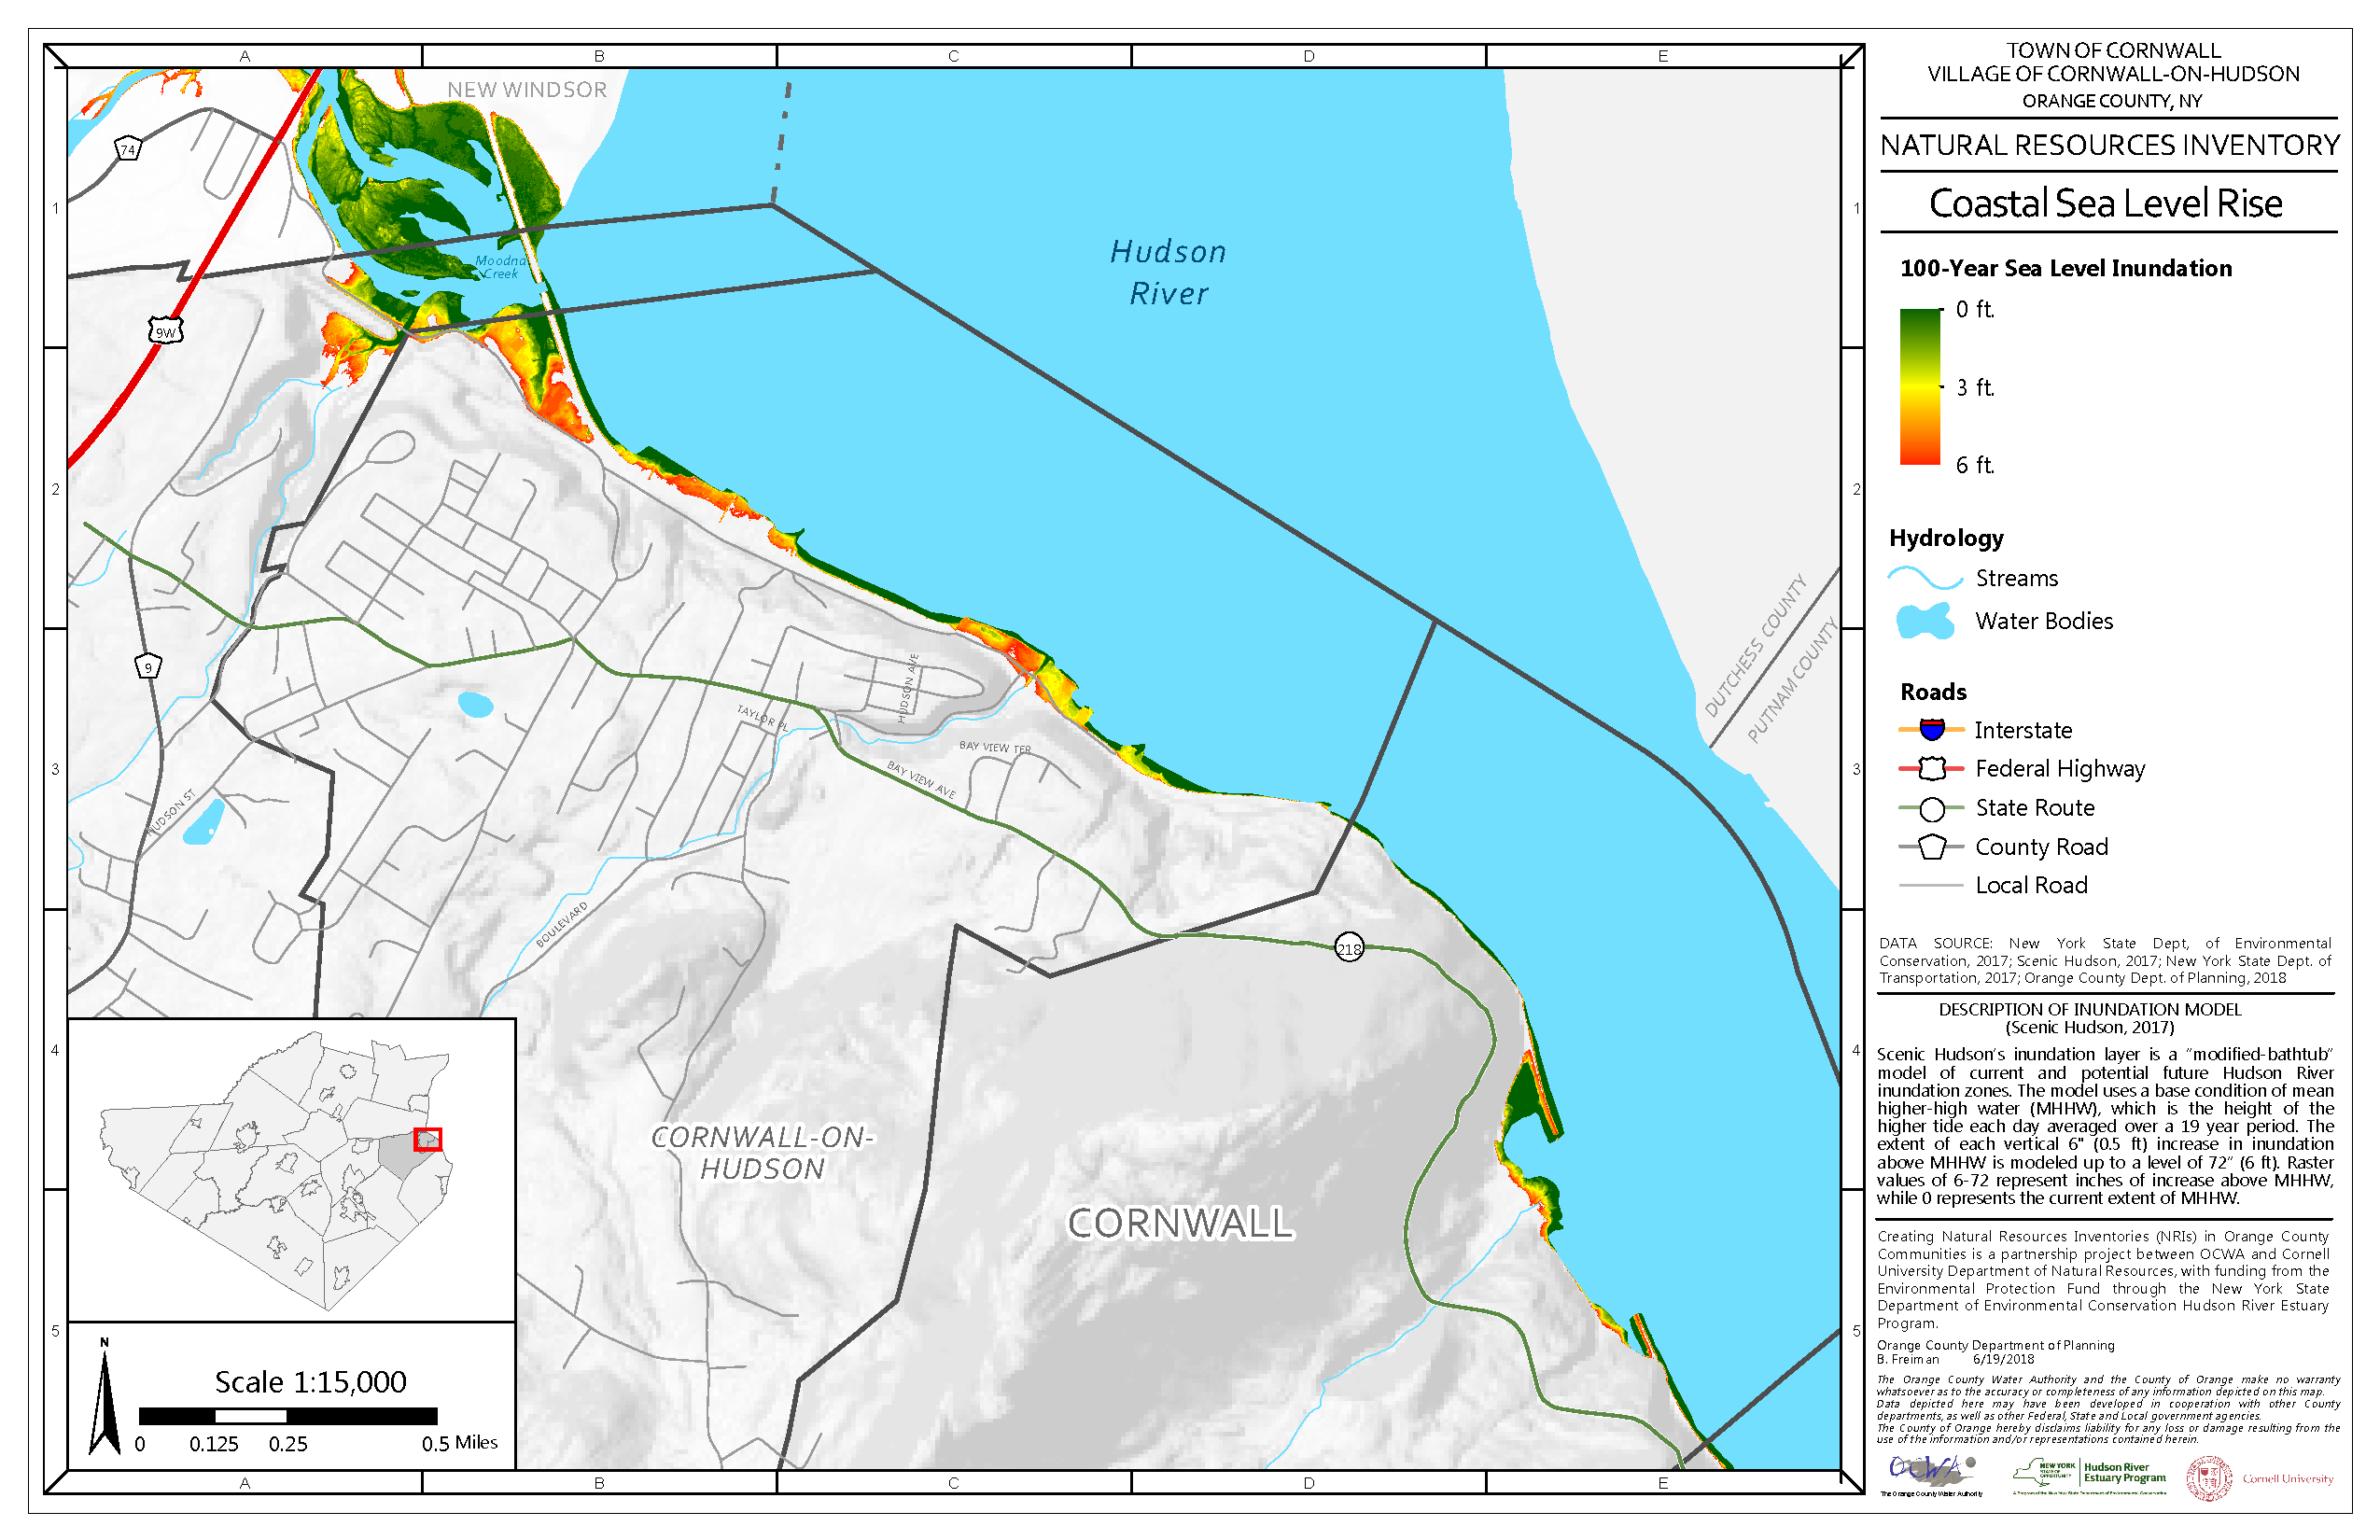
\includepdf[pages=-,fitpaper]{cornwall_maps/CoastalClimateChange.pdf}\label{map:coastalclimatechange}
\subsection*{Coastal Sea Level Rise Map}
The Village of Cornwall-on-Hudson has significant shoreline on the Hudson River 
and is vulnerable to sea level rise. This image shows two important community 
assets: Donahue Memorial Park in the Village and the wastewater treatment plant 
in the Town at the mouth of the Moodna (source: New York Climate Change Science 
Clearinghouse).
\par
The Coastal Sea Level Rise map depicts the areas of future inundation that 
Village and Cornwall residents would experience from a rising Hudson River. In 
a 3-foot sea level rise, 100-year flood scenario (yellow on the map), key 
portions of the wastewater treatment plant are submerged and Shore Road is 
almost inaccessible; we lose roughly half of Donahue Memorial Park to the 
Hudson. In a 6-foot sea level rise scenario (in red), the entire wastewater 
treatment site is in the Hudson and Donahue Memorial Park ceases to exist. Our 
access to the river becomes the train tracks.
\par
In addition to the riverfront inundation modeled in the map, this image shows 
the resulting flooding that would reach inland (orange) as a result of a 6-foot 
sea level rise. 

\subsection*{Becoming a Climate-Resilient 
Cornwall}\label{subsec:climateresilient}
We are already seeing the costly effects of our changing climate and have 
responded to these impacts in different ways. For example, we have protected 
sewage treatment facilities by raising their height, repaired drainage 
destroyed by heavy storms, cleared away left-over storm debris, and cleaned up 
our flooded houses. Understanding the best-case and worst-case scenario 
projections, however, have armed us with the ability to take proactive measures 
to make our community more resilient to the impacts of climate-caused hazards. 
\par
Below is a short list of actions that the New York State Climate Smart 
Communities Program recommends that communities like ours pursue as part of any 
resiliency planning and as a means of responding to the expected federal and 
state mandates for ``strong coastal and floodplain construction standards and 
pre-disaster mitigation planning.''
\begin{enumerate}
    \item Conduct an assessment of municipal and county documents, where 
applicable, to determine the degree to which plans, ordinances, and strategies 
incorporate resiliency planning.
    \item Develop or update a vulnerability assessment to identify ``vulnerable 
    populations, businesses, infrastructure, and natural resources.'' The 
    assessment process assists municipalities with building their knowledge and 
    ability to plan for climate-caused hazards.
    \item Engage the public in identifying the effects of historic storms 
    and make available to the public ``information on the natural and 
    beneficial 
    functions of floodplains, wetlands, and green infrastructure.'' 
    Periodically conduct storm preparedness outreach to residents and 
    businesses.
    \item Develop or update a heat emergency plan. Explore the expansion of 
    cooling centers.
    \item Increase shading in public spaces with trees and other structures.
    \item In the municipal comprehensive plan, reference other plans that 
    address hazard exposure reduction and reduction in property loss, such as a 
    local multi-hazard mitigation plan, floodplain management plan, local 
    waterfront revitalization plan, stormwater management plan, natural 
    resources inventory/plan, etc. Include resilience in the comprehensive 
    plan's mission, vision, or goals.
    \item Incorporate future flooding and preferred adaptation strategies into 
    local planning. Promote best practices and technologies to address flooding.
    \item Right size culverts.
    \item See financial assistance for flood adaptation
    \item Maintain existing natural infrastructure. Use natural vegetated 
    buffers to protect assets from flood risk. Identify and conserve natural 
    areas contributing to stormwater management. 
    \item Encourage building and permitting officials to complete training on 
    retrofitting flood-prone residential buildings.
    \item Implement a program to conserve and reuse water.
    \item Create a source-water protection program.
    \item Establish special area ordinances for habitat preservation. 
    \item Reduce ~\gls{ghg} emissions by supporting and implementing renewable 
    energy and energy efficiency projects.
\end{enumerate}
\nocite{climateexplorer}
\nocite{climatesmart}
\nocite{climateimpactshealth}
\nocite{nysag2014}
\nocite{mhredcstrategic}
\nocite{cscresiliency2014}
\nocite{ocnysenvironmental}
\nocite{degaetano2011}

%*******Proposed Fossil Fuel Infrastructure*****
\section{Proposed Fossil Fuel Infrastructure}
\label{sec:fossil}
\subsection{Proposed Pilgrim Oil Pipelines}\label{subec:pilgrim}
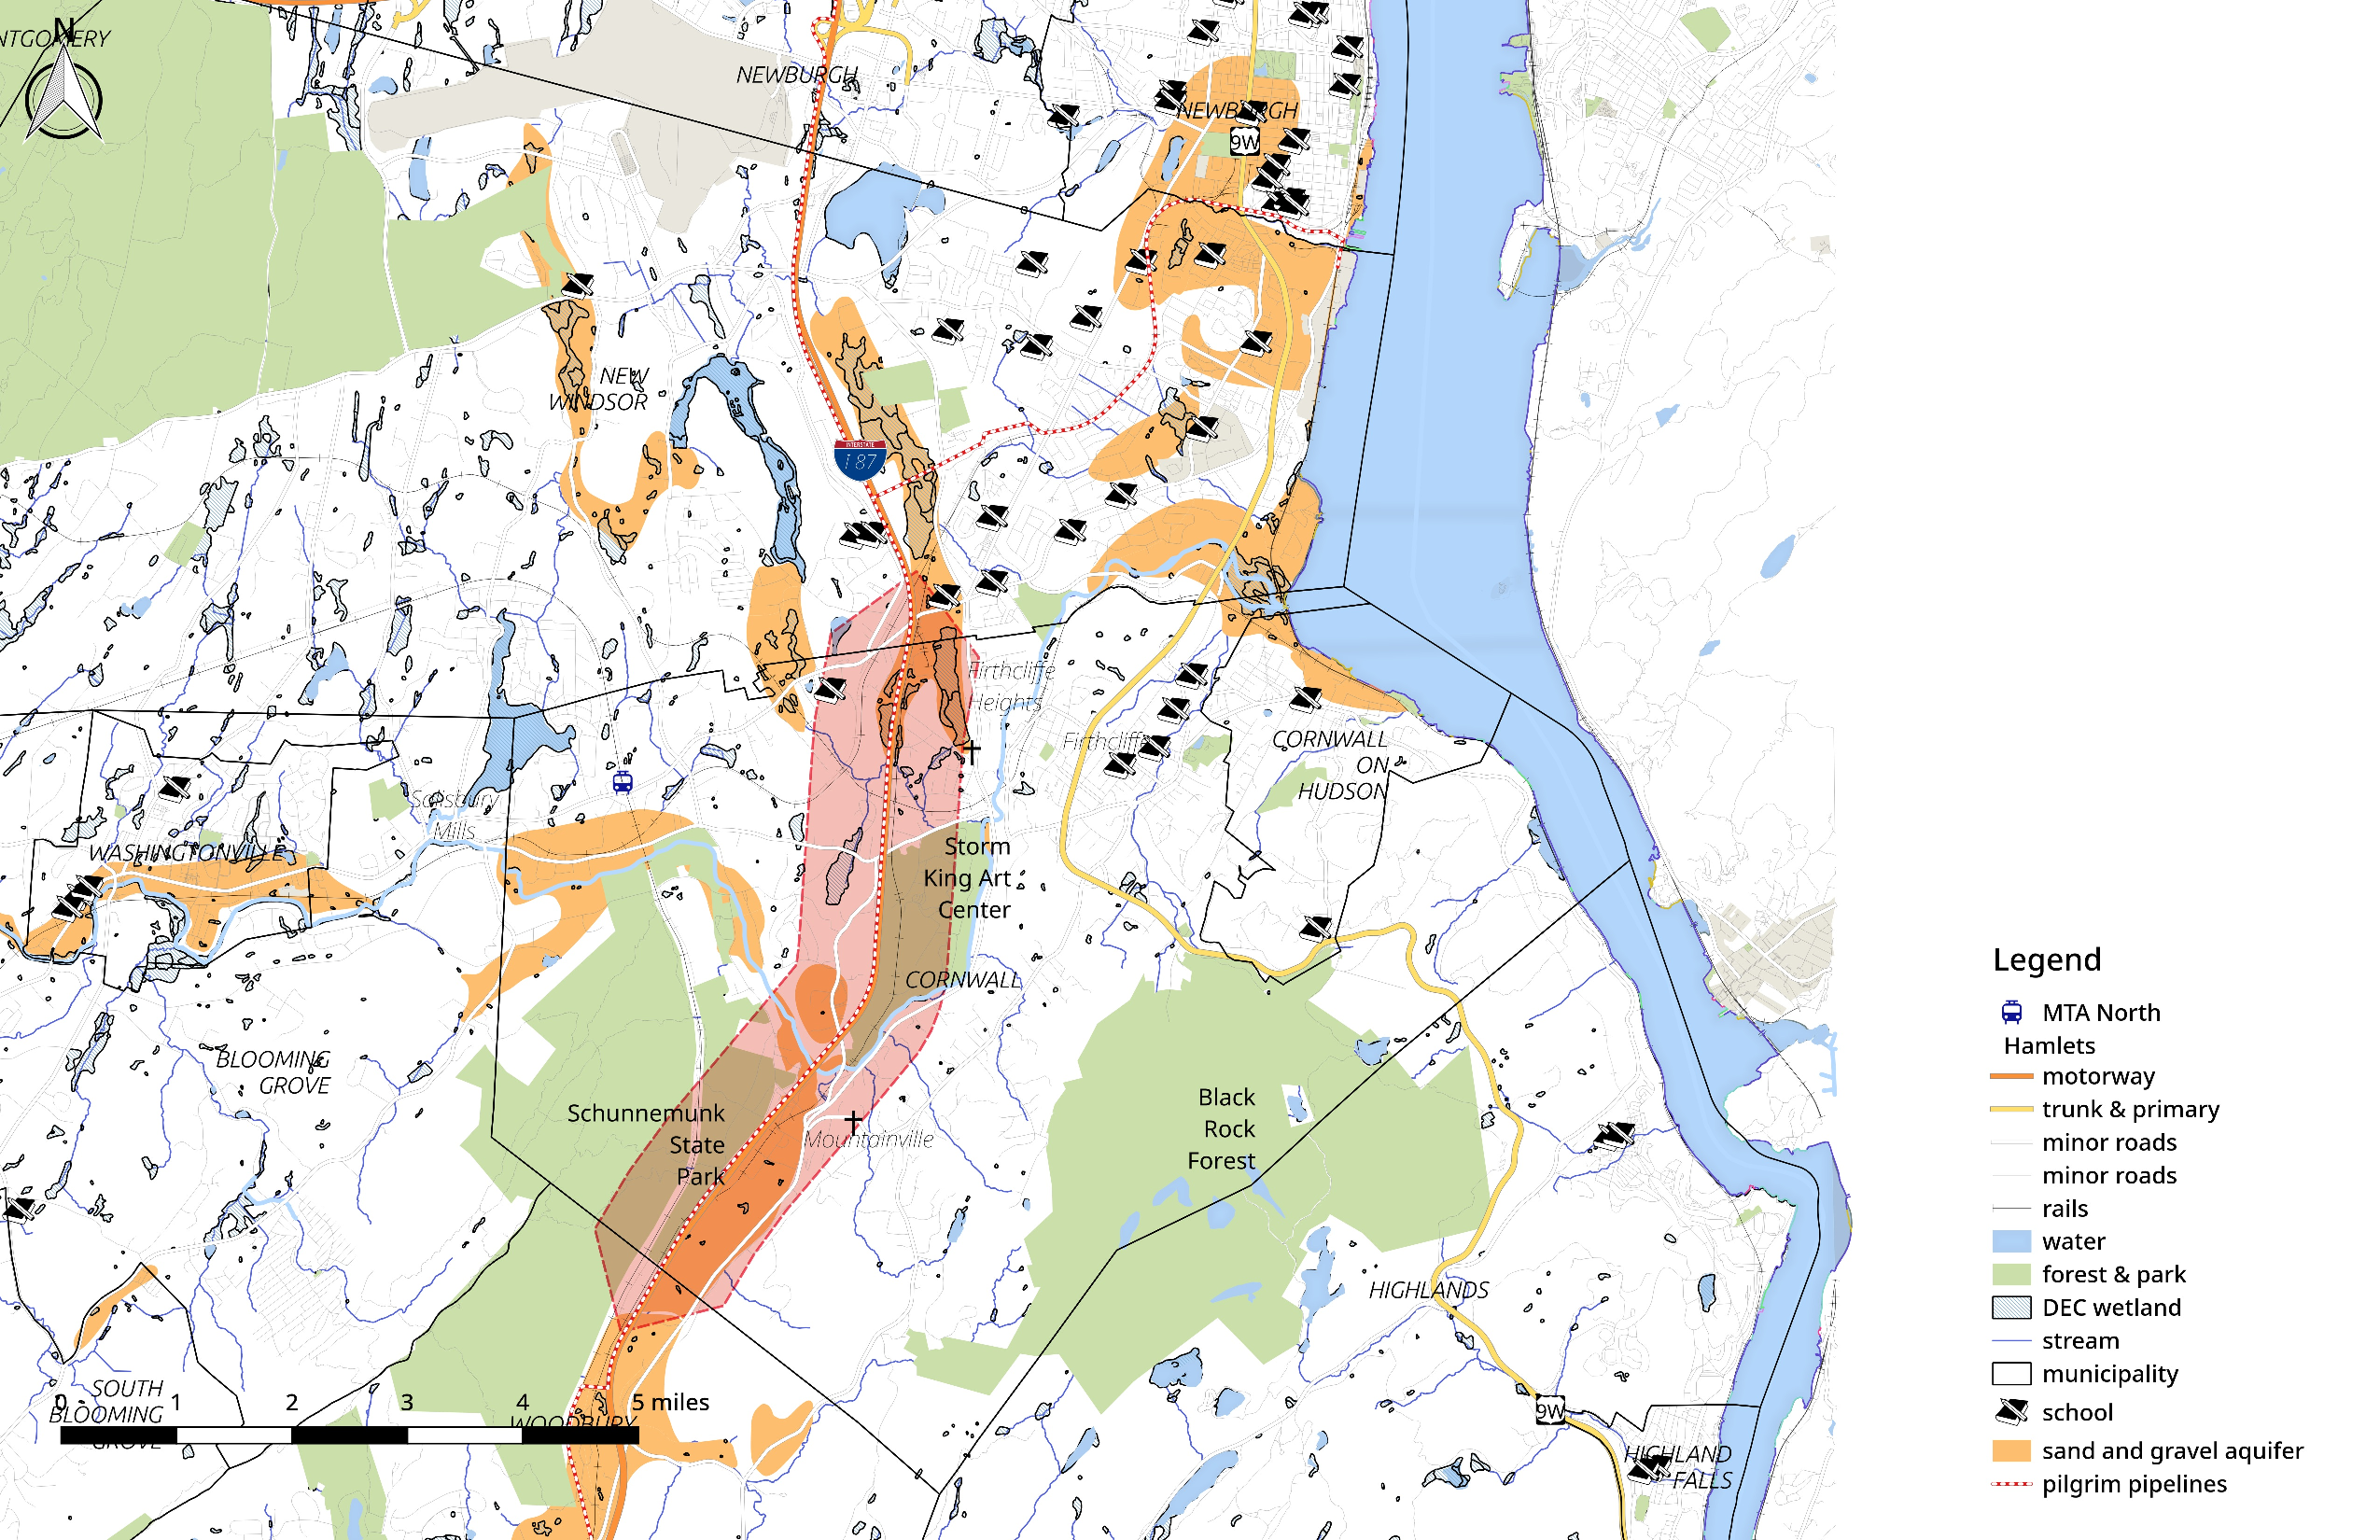
\includepdf[pages=-,fitpaper]{cornwall_maps/proposed_pilgrim_oil_pipelines.pdf}
\label{map:proposedoilpipelines}
This map shows planned fossil fuel infrastructure and its proximity to sand and 
gravel aquifers, public institutions and other important natural areas. The 
proposed Pilgrim Oil Pipelines would carry both refined petroleum products 
(gasoline, diesel, heating oil, and kerosene) and crude oil underground between 
Linden, NJ and Albany, NY along the NYS Thruway. The project’s co-lead 
agencies, \gls{nysta} and \gls{nysdec} determined the project would have 
``potentially significant impact on the environment'' and hence issued a 
``Positive Declaration`` under Article 8 of the Environmental Conservation 
Law. A ''Positive Declaration`` requires a full Environmental Impact Statement 
(EIS) with a public scoping requirement and public comment period. The pipelines 
would be 356 miles long, with 116.4 miles being in New York State, with 5 
laterals, 4 pump stations, 10 meter stations and 35 permanent access roads. 
During construction there would be 50 temporary access roads and 7 major 
construction zones/staging areas. Each pipeline would be 20 inches in diameter 
and have the potential to transport 8.4 million gallons per day (200,000 
barrels/day). The pipelines would cross 257 waterways and would be run very 
close to water supplies of municipalities. There are also 296 (9.2 linear miles)
crossings of wetlands; including 25 crossings of \gls{nysdec}protected 
freshwater wetlands (approximately 19 along mainline pipelines and 6 along 
laterals). If pipelines were constructed more solidly or their leak detection 
systems were better then this might not be an issue. Recent data suggests that 
pipelines are prone to leaking and sometimes days go by before a leak is 
detected and is responded to.

From the south, the pipelines would run adjacent to Schunemunk State Park and 
Storm King Arts Center which are important recreation sites and home to flora 
and fauna. A little less than 5 miles (4.6) of the pipeline would bisect the 
Town’s boundary. Much of the pipelines in Cornwall would be located on top of 
sand and gravel aquifers. The pipeline also traverses across 4 waterways in 
Cornwall and 5 points that are designated as high yielding well sites would be 
within one mile of the proposed pipelines. Two churches and the Cornwall High 
School are within a 0.5 mile risk zone as can be seen on the map. The half mile 
risk zone was added to the map to give viewers an idea off how close they would 
be to the dangers of a leak or an explosion.

In the Town of New Windsor, the lateral would run adjacent to the Quassaick 
Creek which is an important habitat for eel species. Much of the pipelines’ path 
would be built on top of a sand and gravel aquifer which is described as 
“Stratified clay and silt with no or thin layers of sand and gravel at land 
surface and below the water table”. A spill on top of a sand and gravel aquifer 
would risk serious contamination of the groundwater.

\subsection{Proposed Anchorage Sites on the Hudson 
River}\label{subsec:anchorages}
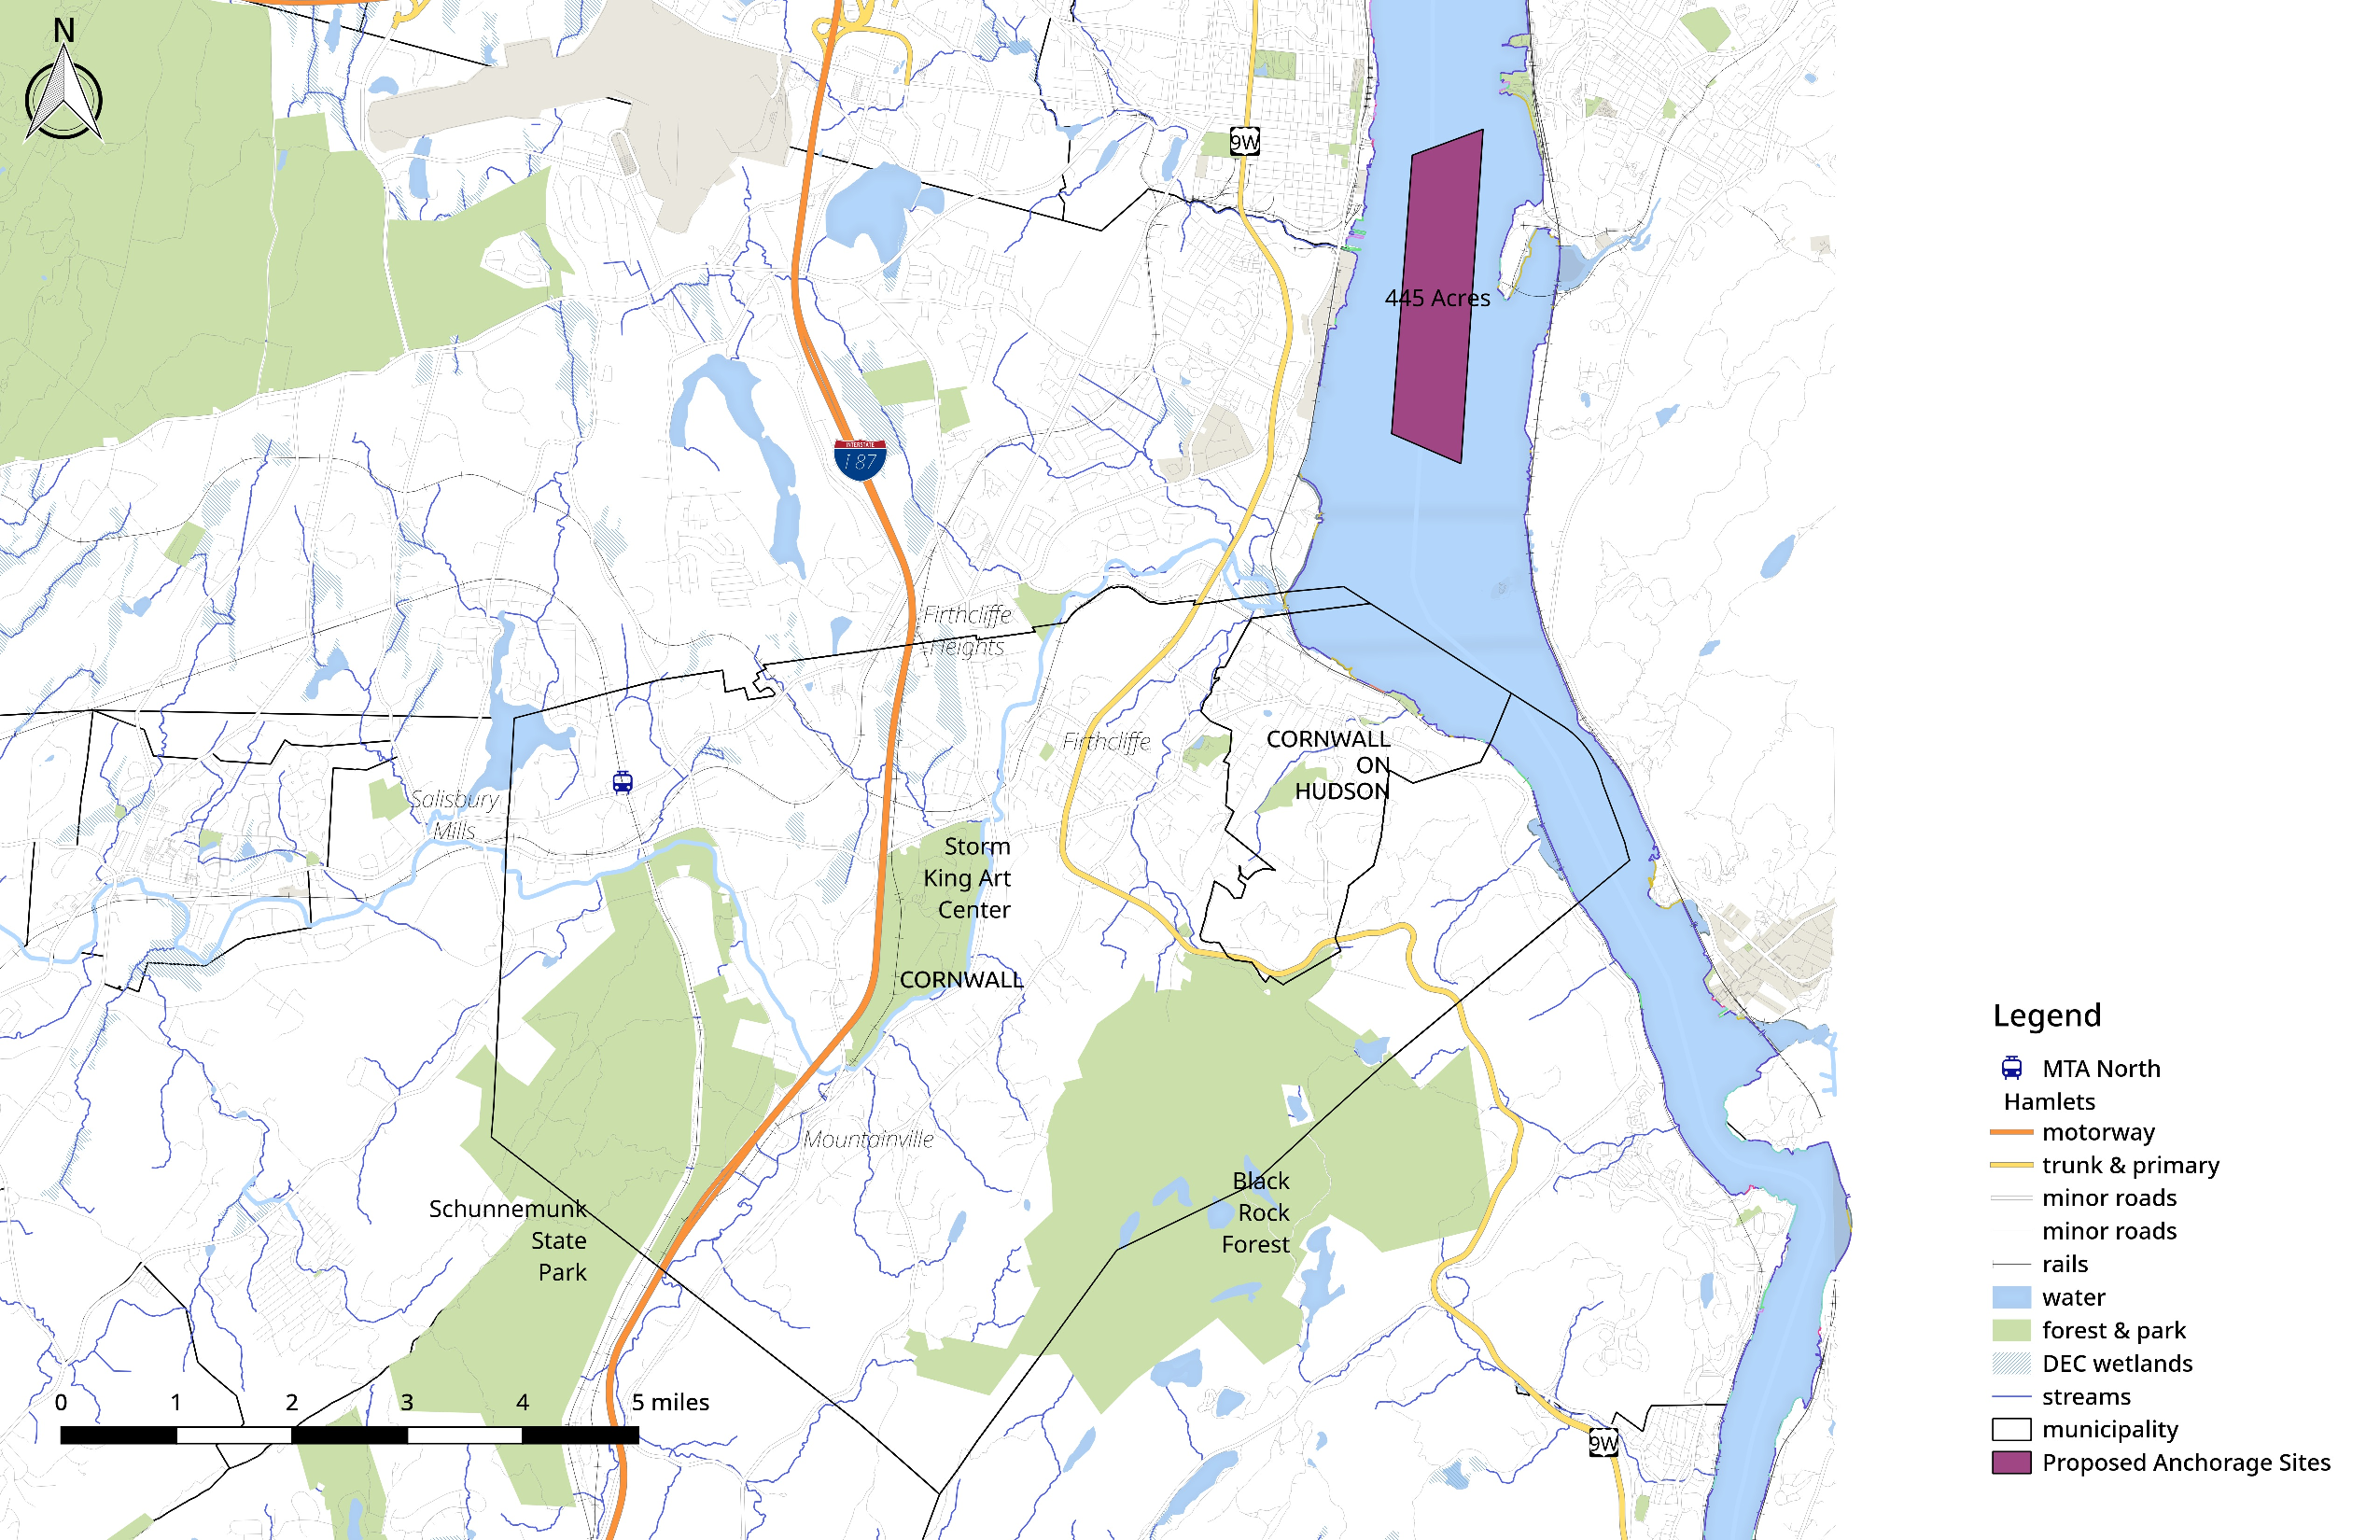
\includepdf[pages=-,fitpaper]{cornwall_maps/proposed_anchorages.pdf}\label{map:proposedanchorages}
This map displays two of the 42 long-term proposed anchorage sites on the Hudson 
River that was submitted by the The Maritime Association of the Port of New 
York/New Jersey to the US Coast Guard in January 2016. The lifting of the oil 
export ban has increased barge traffic on the Hudson River, increasing the risk 
of an accident. The Newburgh hub would have room for a total of 8 barges, with 
space for 5 barges being moored adjacent to the City of Newburgh and 3 moored 
north of the Newburgh/Beacon Bridge. The first area of anchorage sites would 
make 445.34 acres of the Hudson available to barges and the latter would make an 
additional 305 acres of the Hudson available. These barges most likely will 
transport oil and environmental groups have warned that besides the risk of 
spills and explosions that this will turn the Hudson River into a parking lot. 
Due to backlash from engaged citizens, the Coast Guard scrapped the proposal and 
convened a Ports and Waterway Safety Assessment (PAWSA). Multiple workshops were 
held to gain stakeholder insight and plan for a safe Hudson River. Furthermore, 
Governor Andrew Cuomo signed a bill in October, 2017 which gives the 
\gls{nysdec} authority to regulate oil barges on the Hudson River and instructs 
the agency to enact ''tanker avoid zones``.


%********************Land Use******************
\section{Land Use}
\label{sec:Landuse}
\subsection{Farm Soils and Agriculture Parcels}
\subsection{Land Cover}

%\subsection{Figures}
%There will be some figures here maybe.

%References%%%%%%%%%%%%%%%%%%%%%%%%%%%%%%%%%%%%%%%%%%%%%%%%%%%%%%%%
\bibliographystyle{plainnat}
\section{References}
\begingroup
\renewcommand{\section}[2]{}%
%\renewcommand{\chapter}[2]{}% for other classes
\bibliography{bibliography}
\endgroup

%Appendix%%%%%%%%%%%%%%%%%%%%%%%%%
\section{Appendix}
\label{sec:Appendix}

%Glossary%%%%%%%%%%%%%%%%%%%%%%%%%%%%%%%%%%%%%%%
%\printglossary[type=\acronymtype]
\section{Glossary and Acronyms}
\glsaddall
\renewcommand{\glossarysection}[2][]{}
\printglossary

\end{document}
